\section{Foraging Simulation}
\subsection{Foraging Simulation Results}
\begin{figure}[!htb]
    \centering
    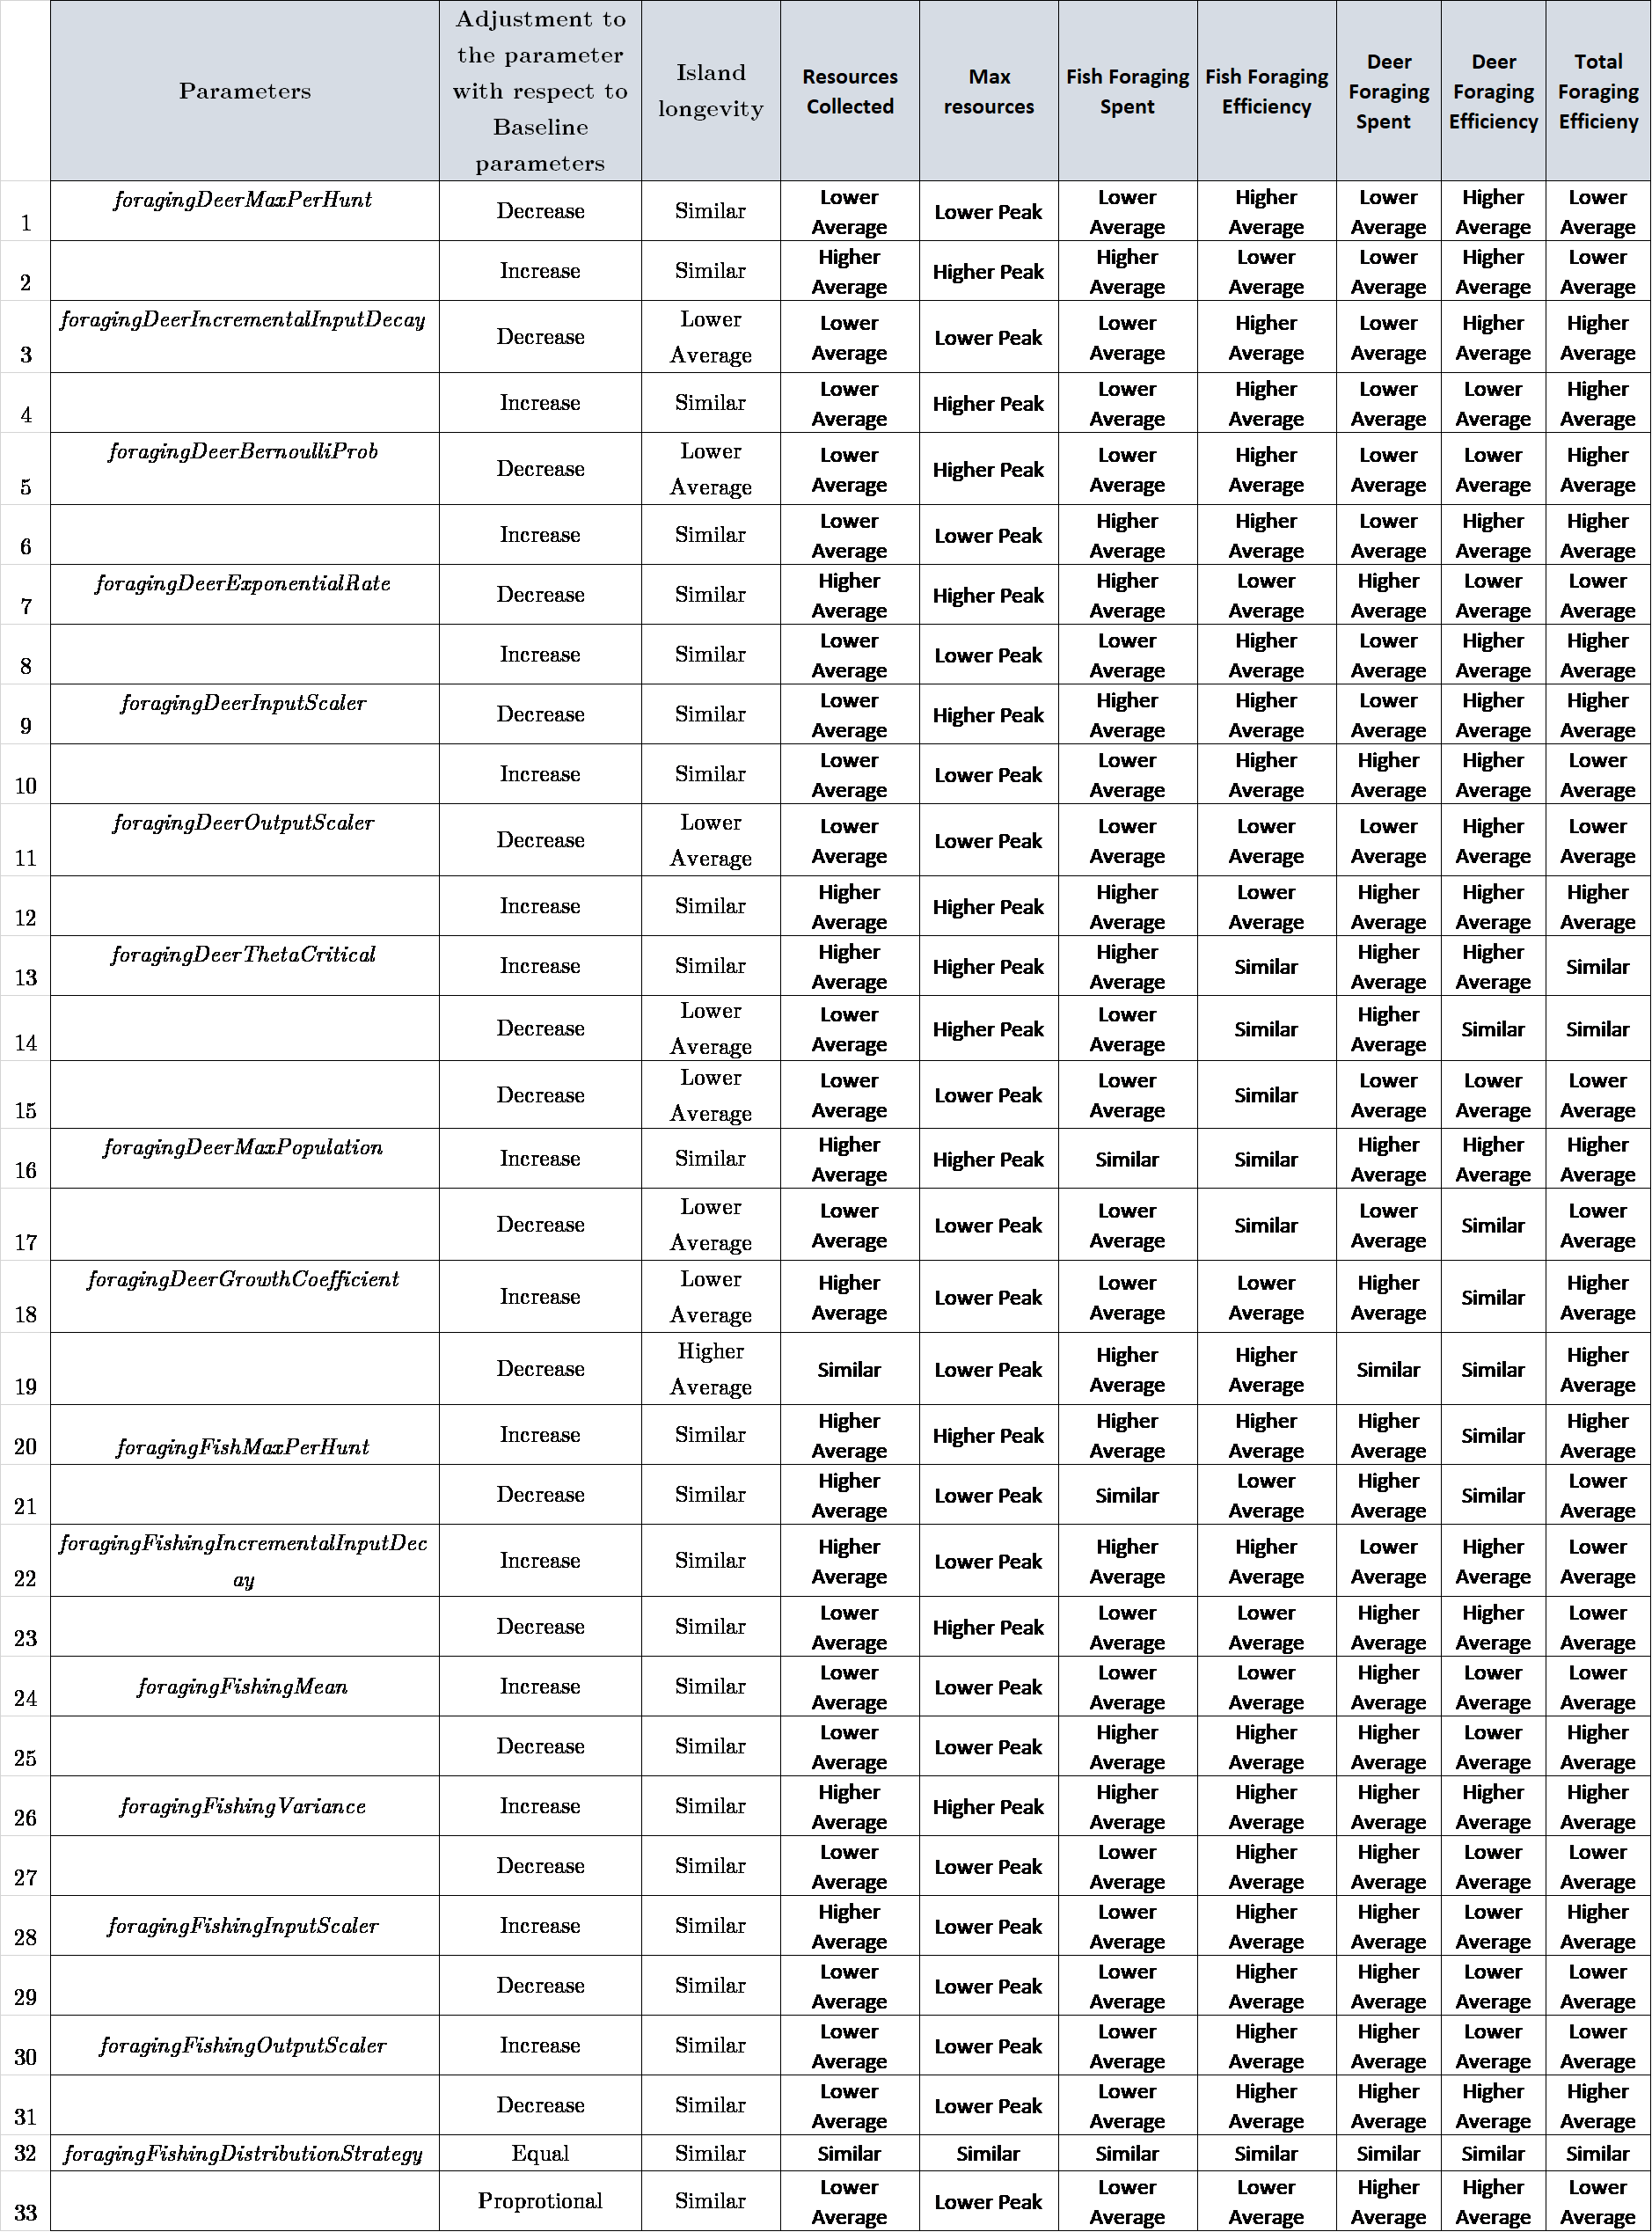
\includegraphics[width=1\textwidth]{16_results_and_eval/images/ForageCommonSim.png}
    \caption{Simulation results for Foraging Parameters using the Environmental metrics of the Archipelago.}
    \label{fig:Resource}
\end{figure}
\subsection{Discussion on Simulation Results}
The simulation for foraging has been completed by adjusting a single environmental parameter whilst fixing the rest and comparing how the metrics change relative to the baseline, examined in earlier sections. For example, in Figure \ref{fig:Resource} the first test involved decreasing the parameter of \texttt{foragingDeerMaxPerHunt} and recording the change observed on the metrics. The tests were run thrice so that extreme scenarios could be mitigated to some extent. If two consecutive tests returned similar results, the result was then recorded. Our findings are presented in Figure \ref{fig:Resource}. The list of metrics recorded was larger, but some were discarded because no strong correlation was visible and others were just irrelevant. 

Starting with \texttt{foragingDeerMaxPerHunt}, we can see an increase in the deer foraging efficiency which could be explained easily as less teams choose to forage when there’s a lower maximum number of deer that can be caught; so those that do have a high efficiency. This can also explain why average resources spent in deer hunting are lower which is caused by less teams choosing to be involved in deer hunting. At the same time, however, an increase in the maximum number of deer per hunt can also cause the deer foraging efficiency to increase. That’s because there are more deer out available for hunting. The same applies for \texttt{foragingFishMaxPerHunt} where similar behaviour is observed. In both cases, results are affected by random variables and distributions that exist throughout the implementation of foraging in environment and thus, at different instance, results will vary.


Same principles apply for \texttt{foragingDeerMaxPopulation} and \texttt{foragingDeerBernoulliProb}. Both of these parameters influence the population of Deer and thus, a higher population will lead to generally larger efficiencies as can be confirmed in Figure \ref{fig:Resource}. In addition, a higher max resource peak can be observed and in general, agents seem to be more prosperous. The opposite is valid when we decrease populations and parameters that affect growth and probability of catching a deer or a fish. It is observed that there can be exceptions and some metrics shift to a direction we did not expect; such as the deer hunting efficiency when we increase \texttt{foragingDeerGrowthCoefficient}. Again, this can be due to the agents’ dynamics not being able to detect some of the probabilistic discrepancies that exist in the game.

The main observation that can be made when comparing fish and deer hunting is that there is usually a much higher engagement in fishing, compared to deer hunting. That can be observed by the trends present on Figure \ref{fig:Resource}. especially when deer hunting parameters are adjusted in a way to encourage deer hunting. Even in that case, there might be an increase in the average resources spent on fishing, telling us that fish may be more attractive to agents. Multiple guess can be made as to why that happens, but it may be very well dependent on the agents’ risk level tolerance and not being able to comprehend a population model, due to its complexity.

In general, the results are as expected if we can confidently blame some of the mismatches between empirical observations and expected ones onto randomness. Nevertheless, the current system may be too complex for the agents to analyse and create a knowledge base of skills that could result in more effective foraging. To conclude, due to a very narrow testing period, the analysis is not complete and should be further evaluated; possibly by examining another set of metrics and correlations that can exist between parameters. Also, the number of simulations is important and each individual test needs to be run multiple times in order to minimise the variance on some of the parameters. 






